\documentclass[11pt]{article}

\usepackage{float} % [H] option for tables
\usepackage{booktabs} % table ruling
\usepackage{framed} % Frame for listings
\usepackage{fullpage} % Use the full page
\usepackage{color}
\usepackage{tikz}
\usepackage{matlab-prettifier} % Matlab
\setlength\parindent{0pt} % No indentation


% Headers
\usepackage{fancyhdr}
\setlength{\headheight}{15.2pt}
\pagestyle{fancy}
\setlength\headsep{30pt}
\lhead{Youssef Beltagy and Samuel Hunter}   					%  Your name on the left header.
\chead{\textsc{Lab 3}}			%  Title in the center.
\rhead{\today}							%  Date on the right header.

% Matlab blocks
\lstset{
  style              = Matlab-editor,
  basicstyle         = \mlttfamily,
  mlshowsectionrules = true,
  escapeinside={//}{\^^M},
}

% Cover Page Settings
\title{
    \textsc{Lab 3 Report: Fourier Series and Gibbs Phenomenon}
}

\author{
    \Large{Youssef Beltagy and Samuel Hunter} \\
    \large \textsc{AUT21 BEE 235}
}

\date{\today}



%--------------------------------------------
%%%%%%%%%%%%%%%%%%%%%%%%%%%%%%%%%%%%%%%%%%%%%%%%%%%%
% END OF THE PREAMBLE AND BEGINNING OF THE ACTUAL DOCUMENT
%%%%%%%%%%%%%%%%%%%%%%%%%%%%%%%%%%%%%%%%%%%%%%%%%%%%
%--------------------------------------------

\begin{document}


\maketitle % Make the cover page
\pagebreak


\section{Abstract}

In this lab, we analyze a couple of signals and synthesize them using the fourier series.
We analyzed a trumpet sound and a square wave signal.
We observed and recorded how synthesized signals fare compared to original ones.

% =================================================
% PART 1
% =================================================
\section{Part 1 --- Signal Synthesis}

In this section we analyze and synthesize a trumpet sound using fourier series.

\subsection{Estimating the Fundamental Frequency}

After loading and plotting the pre-recorded trumpet sound signal onto a graph, we measured the coordinates of two different peaks.

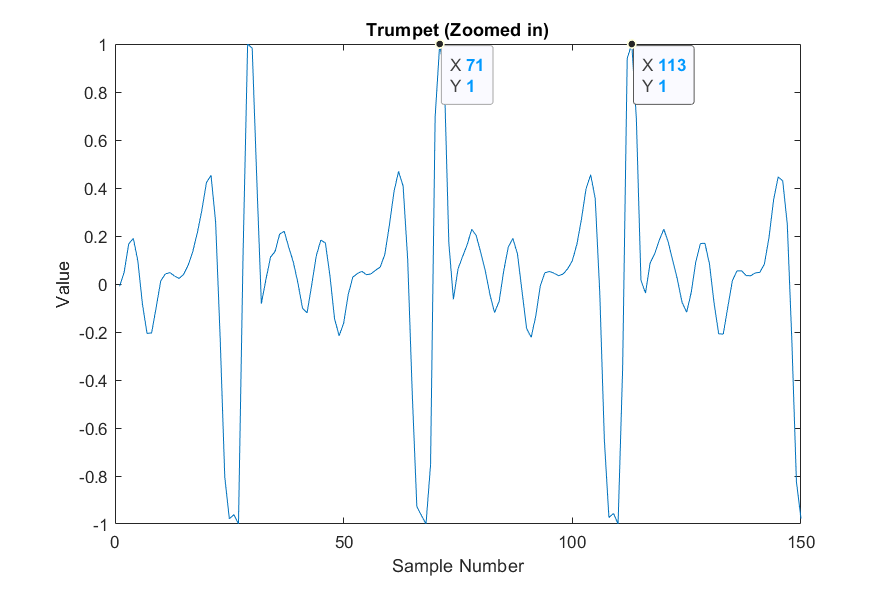
\includegraphics[width=\textwidth]{trumpet_zoomedin.png}

\begin{table}[H]
	\centering
	\begin{tabular}{cccc}\toprule
		Peak No. 1 & Peak No. 2 & Period (\# of samples) & $F_0 (Hz) = F_s / (\textrm{\# of samples})$ \\\midrule

		$X_1 = 71, Y_1 = 1.0000$ &
		$X_2 = 113, Y_1 = 1.0000$ &
		$|X_2-X_1| = 42$ &
		$F_0 = 11025 / 42 = 262.5\;Hz$ \\\bottomrule
	\end{tabular}
	\caption{\label{tab:two-peaks}Two sampled peaks of the trumpet sound signal}
\end{table}

The difference between the two peaks is 42 samples.
With a sample rate of $F_s = 11025\;Hz$, the difference is $262.5\;Hz$.\\

We then applied the Fourier transform on the trumpet signal and measured the magnitudes and frequency of the first seven harmonic peaks.
We also included the 0th harmonic (the integral average) for reference.

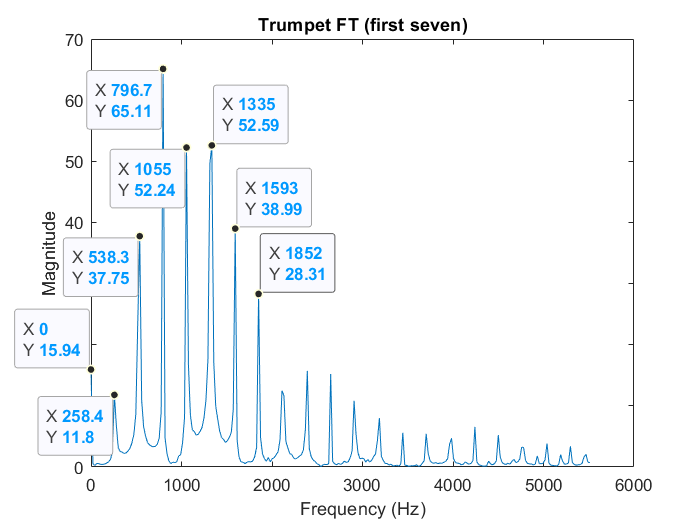
\includegraphics[width=\textwidth]{trumpet_ft_first7.png}

\begin{table}[H]
	\centering
	\begin{tabular}{rrrr}\toprule
		Harmonic & Magnitude & Frequency (Hz) & Frequency Diff (Hz)\\\midrule
		0 & 15.944 & 0  & N/A \\
		1 & 11.795 & 258.398 & 258.398 \\
		2 & 37.749 & 538.330 & 279.932 \\
		3 & 65.114 & 796.729 & 258.399 \\
		4 & 52.244 & 1055.13 & 258.40 \\
		5 & 52.593 & 1335.06 & 279.93 \\
		6 & 38.994 & 1593.46 & 258.40 \\
		7 & 28.305 & 1851.86 & 258.40 \\\bottomrule
	\end{tabular}
	\caption{\label{tab:first-harmonics}7 first harmoncs}
\end{table}

The mean of these differences is $F_0 \; = \; 264.55$ Hz and the median of these differences is 258.40 Hz.
The percent differences compared to our first estimation of 262.5 Hz is 0.78\% and 1.6\% for the mean and median respectively.
The percent differences are small so the mean and median align well with our first estimate.\\

The harmonics all have frequencies which are multiples of $F_0 \; = \; 264.55$ Hz (approximately).
So the average difference between two harmonics is 264.55. It seems musical sounds are
made of multiple harmonics and not just one.\\

Here is the code used in analysis.

\begin{framed}
	\lstinputlisting{signal_synthesis_plot.m}
\end{framed}

\subsection{Signal Synthesis}

To synthesize a new trumpet signal, we recorded the 10 strongest (in magnitude) harmonic peaks.
We ignored the 0th harmonic (when the frequency is 0 Hz) because it will just make the sound louder 
without making it more intelligible and matlab will attenuate the larger magnitude.
We did try adding the 0th harmonic, but it didn't make the sound any better.

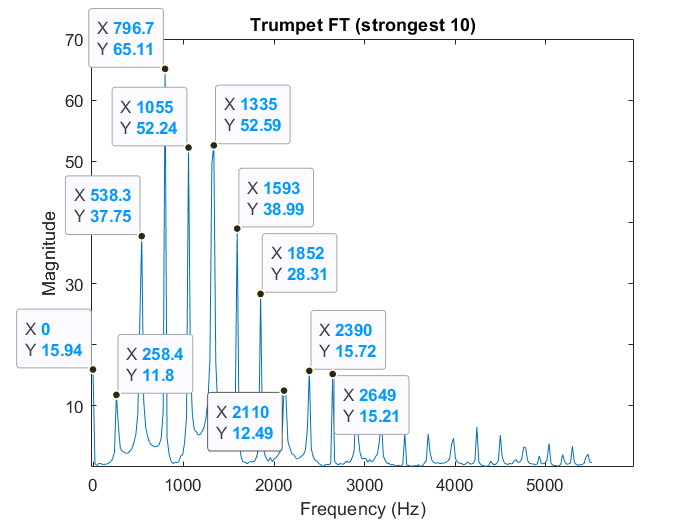
\includegraphics[width=\textwidth]{trumpet_ft_strongest10.png}

\begin{table}[H]
	\centering
	\begin{tabular}{c c c}\toprule
		Peak & Magnitude & Frequency (Hz) \\\midrule
		 1 & 65.114 & 796.729 \\
		 2 & 52.593 & 1335.06 \\
		 3 & 52.244 & 1055.13 \\
		 4 & 38.994 & 1593.46 \\
		 5 & 37.749 & 538.33  \\
		 6 & 28.305 & 1851.86 \\
		 7 & 15.724 & 2390.19 \\
		 8 & 15.208 & 2648.58 \\
		 9 & 12.487 & 2110.25 \\
		10 & 11.795 & 258.398 \\\bottomrule
	\end{tabular}
	\caption{\label{tab:strongest-harmonics}10 strongest harmonic peaks}
\end{table}

We then created a matlab script that summed up 10 sine waves into a $2*F_s$-long vector to synthesize a 2-second long trumpet signal.\\

The synthesized signal sounded much like the pre-recorded trumpet signal
but had zero variance in tone.
The synthesized signal sounded monotonic and had a weird ringing sound.
The synthesized signal may sound better if more harmonics are added.\\

Below is the synthesized signal. It is periodic and doesn't have any variation.
It still has a sinusoidal form.

% Synthesis output
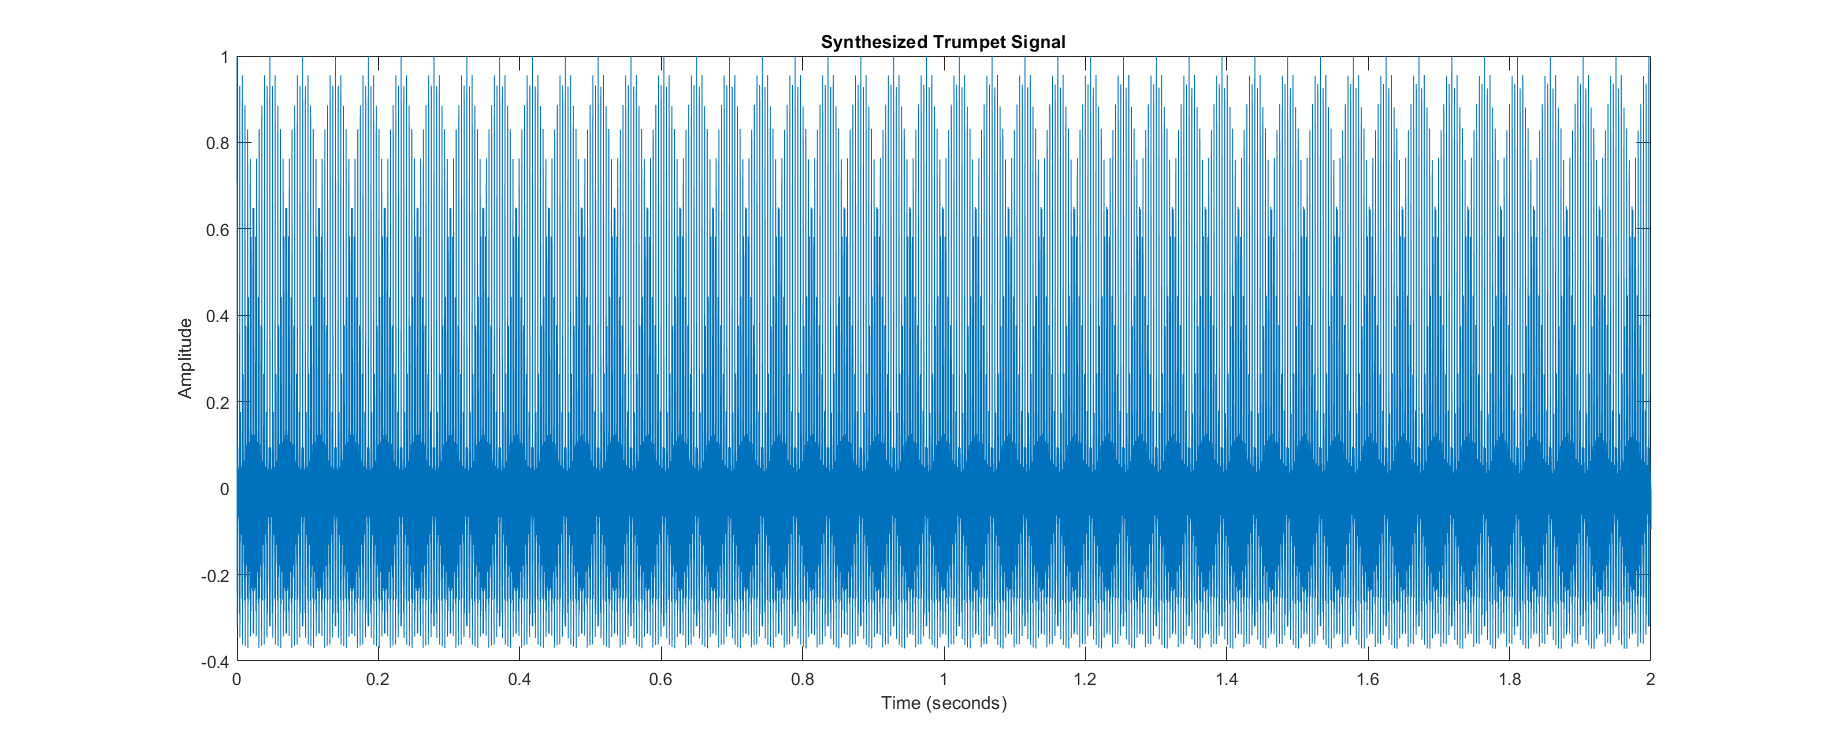
\includegraphics[width=\textwidth]{signal_synthesis.png}

Compared to the original signal, the synthesized signal is missing components.
The synthesized signal seems to mostly contain the dense central part of the original
which you can see in the image below. The other frequencies are truncated.

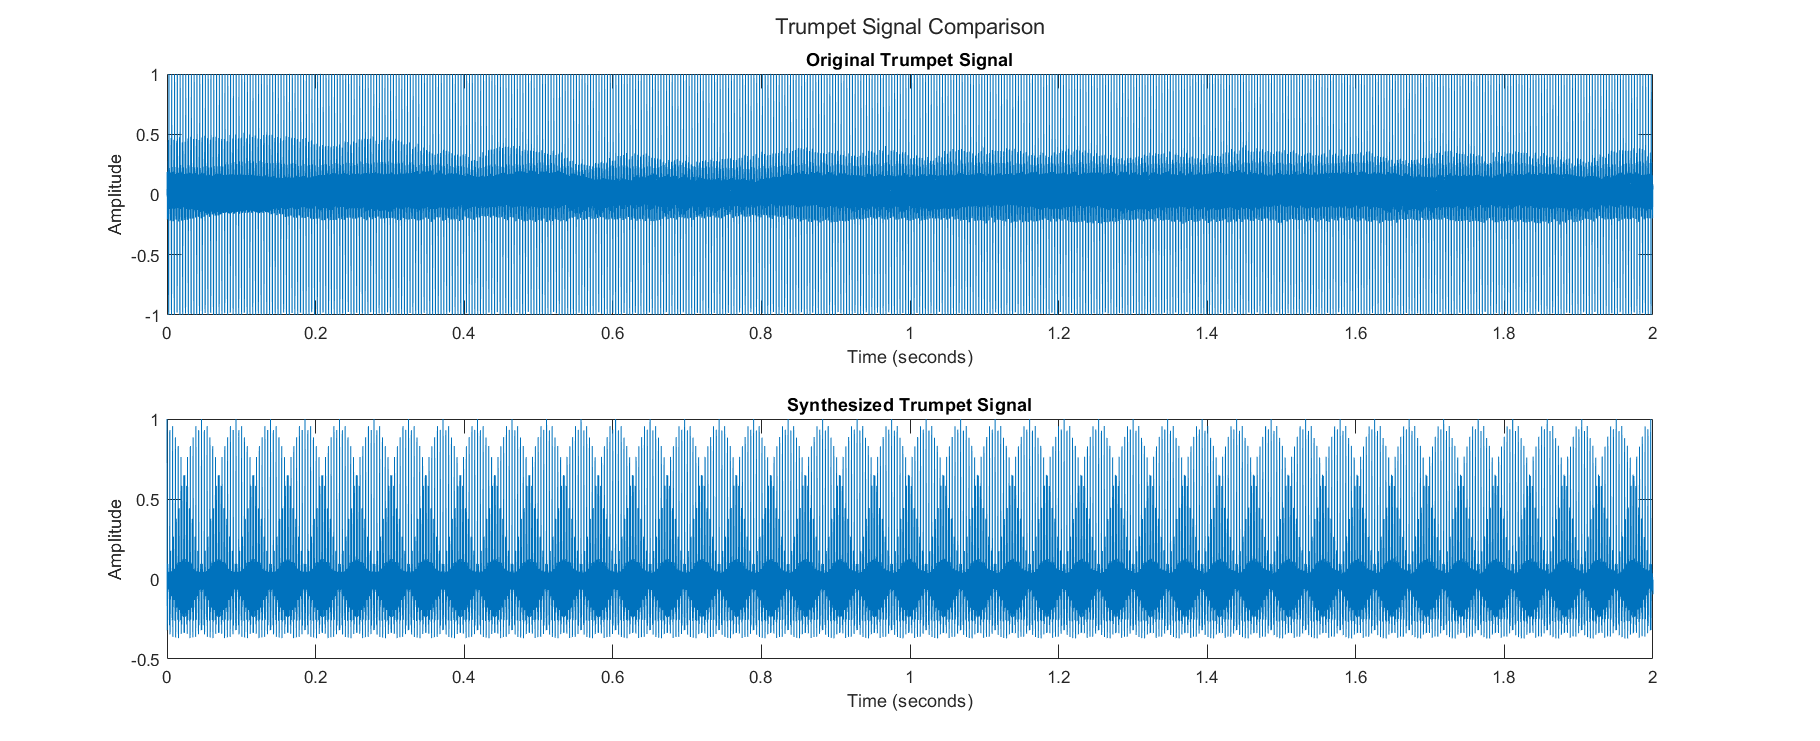
\includegraphics[width=\textwidth]{trumpet_signal_comparison.png}

When we zoomed into the signals, it is clear the two signals are not in phase.
This is because we only used the magnitudes of the coefficients for the fourier series
and didn't consider the phase.\\

The original signal appears smoother than the synthesized signal.
The original signal has values in the range of [-1,1] 
but the synthesized signal only has values in the range of [-0.5,1]. 
The original signal has negative peaks of bigger magnitude than the synthesized signal.
All of these points illustrate how the synthesized signal is missing most components of 
the original. Yet, the synthesized signal is adequately similar to the original for
us to identify it.


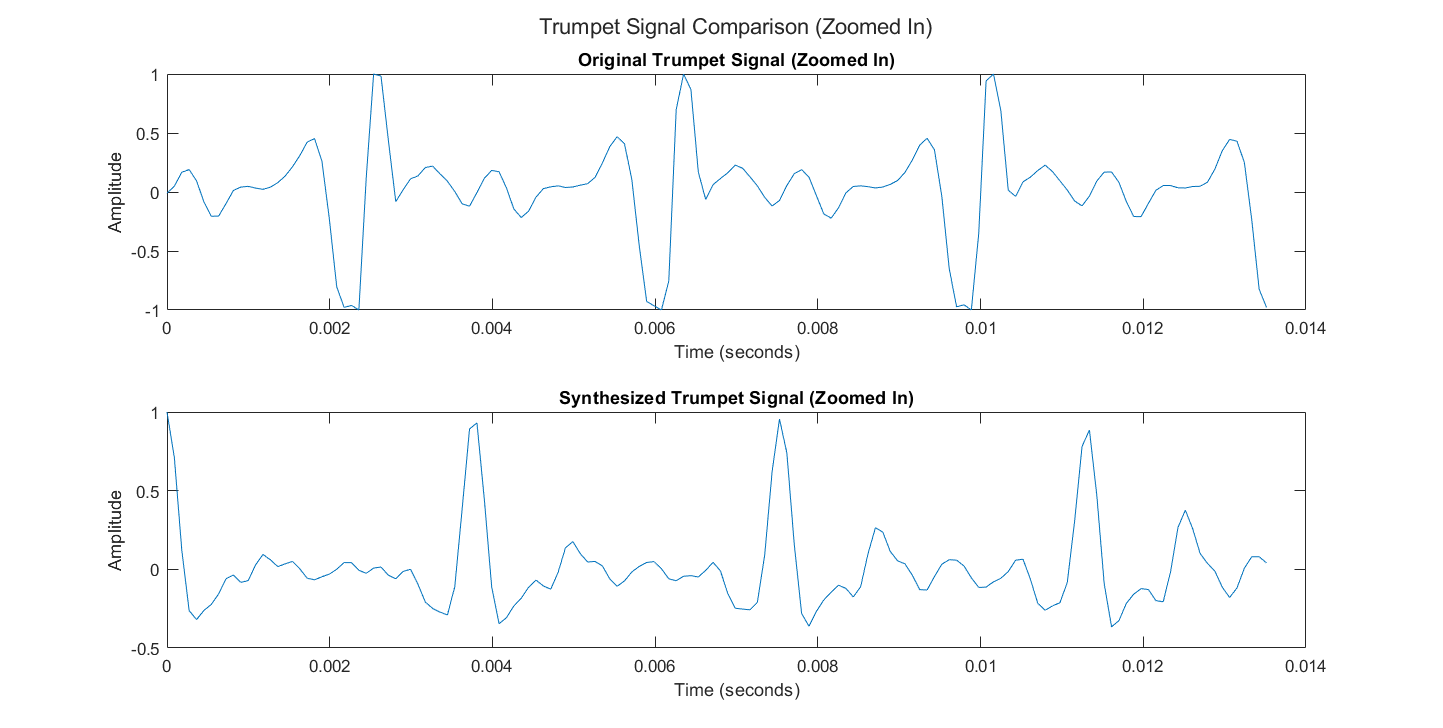
\includegraphics[width=\textwidth]{trumpet_signal_comparison_(zoomed in).png}


% Synthesis code
\begin{framed}
	\lstinputlisting{signal_synthesis.m}
\end{framed}


% =================================================
% PART 2
% =================================================
\pagebreak
\section{Part 2 --- Fourier Series Approximation of a Square Wave}

In this section, we synthesized a square wave signal using a fourier series.
When the number of coefficients is low, the synthesized signal displays the Gibbs
phenomenon where the signal overshoots and undershoots at sharp transitions.

\subsection{C\_k Phase and Magnitude}

We generated and plotted the C\_k coefficients of the fourier series
we used to synthesize the square wave.\\

Below you can see the magnitudes and phases of the coefficients.

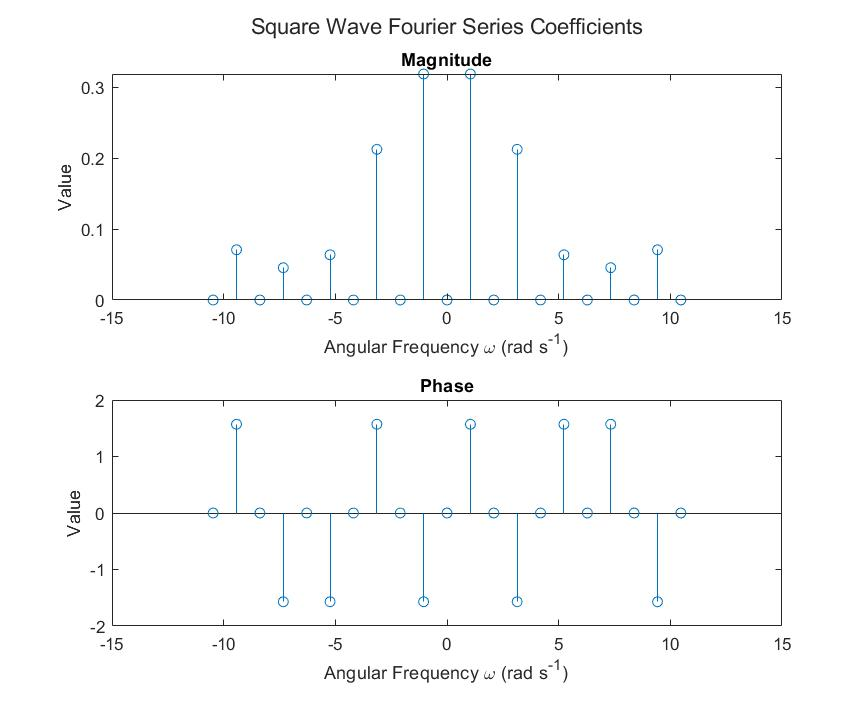
\includegraphics[width=\textwidth]{ck_values.png}

\begin{framed}
	\lstinputlisting{gibbs.m}
\end{framed}

\subsection{Square Wave Synthesis}

We developed a function that generates an approximation of a square wave
given the time of the signal and the K\_{max} of the coefficients.

\begin{framed}
	\lstinputlisting{squarewave.m}
\end{framed}

\pagebreak
\subsection{Square Wave Plots}

We plotted the output from our synthesizing function.
Clearly as K\_{max} increases, the synthesized signal becomes
more similar to the original.

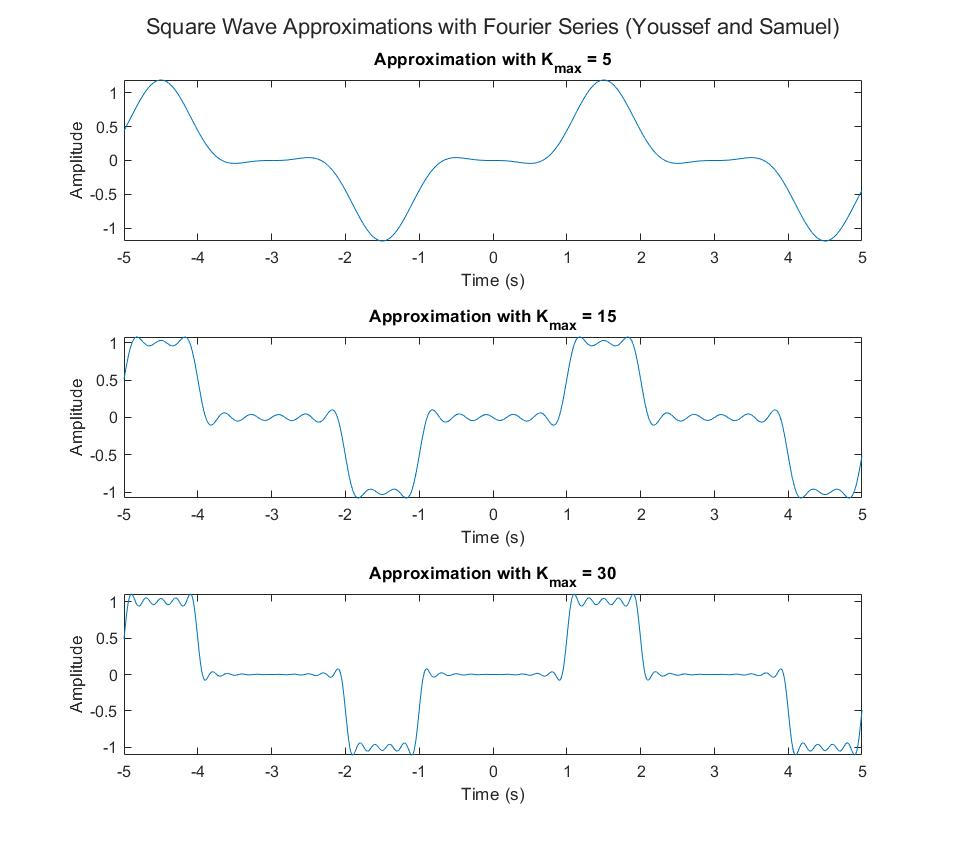
\includegraphics[width=\textwidth]{squarewaves.png}

\begin{framed}
	\lstinputlisting{squarewave_plot.m}
\end{framed}

\subsection{Gibbs Phenomenon}

The plots didn't demonstrate the phenomenon enough,
so we wrote a script to generate a video of the synthesized signal
as k\_{max} increases.\\

When K\_{max} is less than 500, the Gibbs phenomenon is clear.
The signal rings (overshoots and undershoots) at sharp transitions.\\

Between K\_{max} = 400 and K\_{max} = 500, the ringing decreases.
When K\_{max} rises above 500, the Gibbs phenomenon disappears.
After that it appears again; then it disappears again; 
then it appears again, and the process repeats.

\begin{framed}
	\lstinputlisting{squarewave_video.m}
\end{framed}

\section{Conclusion}

We used the fourier transform to analyze a trumpet sound.
We then used the strongest harmonics of the trumpet to synthesize a trumpet sound using the fourier series.
By summing cosines mapping to the highest-magnitude harmonics, we can generate a signal that mimics the timbre of a sound piece.\\

We synthesized a square wave using its fourier series coefficients and compared it to the original signal.
Fourier series can be used to generate signals with sharp transitions.\\

Because the synthesized signals are truncated fourier series, they have some issues
like the Gibbs phenomenon or imperfect representations of the signal.
The synthesized trumpet sound has zero variance in tone and is not able to replicate any ``wibbly-wobbly'' sound that appears because of smaller frequencies in the sample.
The square wave displayed the Gibbs Phenomenon even when hundreds of frequencies were used.\\

Nonetheless, a Fourier series can generate sound tables that can be used by synthesizers and other digital audio tools as a base for instruments.

\end{document}
